\documentclass[16pts]{report}
\usepackage[utf8]{inputenc}
\usepackage[T1]{fontenc}
\usepackage[francais]{babel}
\usepackage{xcolor}
\usepackage[hyphens]{url}
\usepackage[hidelinks]{hyperref}
\usepackage{amsmath}
\usepackage{graphicx}
\usepackage{geometry}
\usepackage{textcomp}
\hypersetup{hypertexnames=true}
\geometry{hmargin=2.5cm,vmargin=1.5cm}

\usepackage{float} %Option H pour les figures, utile.

%\maketitle
%\clearpage

\begin{document}
\bibliographystyle{unsrt}
\nocite{*}

\chapter{Développement}
\label{cha:Développement}

\section{Choix technologique}
\label{sec:Choix technologique}

Dès les premières réunions avec notre client, nous avions discuté du langage à 
utiliser pour concevoir l'application. La première proposition était d'utiliser 
le langage C. En effet, vu que cette application a pour but d'être adoptée par 
la communauté Linux, il aurait été judicieux de la coder avec le langage 
qu'elle préfère. Dans un premier temps, nous avions pensé à la réaliser
en Java, mais ce langage n'est pas très apprécié par cette communauté.

Ensuite, après avoir bien avancé dans la recherche de notre existant, nous 
avons trouvé une bibliothèque en Python permettant de manipuler les options 
d'un noyau Linux. Dans une optique d'homogénéité, nous avons décidé de réaliser 
toute notre application en Python et cela ne posait pas de problèmes au client.

En ce qui concerne l'utilisation de la bibliothèque Python que nous avons 
trouvée, nous avions le choix entre refaire cette gestion nous-mêmes, ce qui 
aurait pris une grande partie de notre temps de développement et celui-ci 
était très limité. Nous avons donc décidé de nous servir de cet existant 
afin de pouvoir nous concentrer sur d'autres tâches comme l'affichage 
des options en conflits.

\section{Cycle de vie}
\label{sec:Cycle de vie}

\begin{figure}[H]
	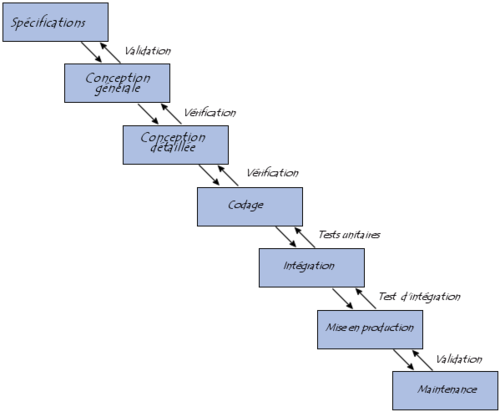
\includegraphics[scale=0.7]{../illustrations/cycle_cascade.png}
	\centering
	\caption{Schéma du cycle en cascade}
	\label{fig:CycleCascade}
\end{figure}

Ce projet a eu un cycle de vie en cascade avec retour. En effet, durant toutes 
les phases de notre projet, nous avons soumis notre travail à vérification 
et validation afin de pouvoir être en accord avec notre chargé de TD et notre 
client. L'utilisation de ce cycle de développement n'a pas été un choix, car 
il était imposé par le formalisme de cet enseignement. Cependant, celui-ci a 
été très utile, car il nous a permis de réaliser une analyse conséquente dès 
le début du projet afin de définir précisément les besoins de notre client.

\end{document}
